% ថ្នាក់ទី ១១ (វិទ្យាសាស្ត្រ) · ជំពូកទី ២ · មេរៀនទី ២ · សៀវភៅទំព័រ ៧២–៨៨
\chapter{អនុគមន៍លោការីត}

\begin{objBox}[វត្ថុបំណង]
\begin{enumerate}[1]
  \item សង់ក្រាបនៃអនុគមន៍លោការីត
  \item ដោះស្រាយសមីការនិងវិសមីការលោការីត ។
\end{enumerate}
\end{objBox}

\section{ក្រាបនៃអនុគមន៍លោការីត}

\begin{example}[ឧទាហរណ៍ ក]
សង់ក្រាបនៃអនុគមន៍ $y = 4^x$, $y = \log_4 x$ និងបន្ទាត់ $y = x$ ។

តារាងតម្លៃត្រូវគ្នានៃ $x$ និង $y$
\[
\begin{array}{|c|c|c|c|c|c|}\hline
x & -2 & -1 & 0 & 1 & 2\\ \hline
y = 4^x & 0.06 & 0.25 & 1 & 4 & 16\\ \hline
\end{array}
\]
\[
\begin{array}{|c|c|c|c|c|c|}\hline
x & 0.25 & 0.50 & 1 & 2 & 4\\ \hline
y = \log_4 x & -1 & -0.50 & 0 & 0.50 & 1\\ \hline
\end{array}
\]
\begin{center}
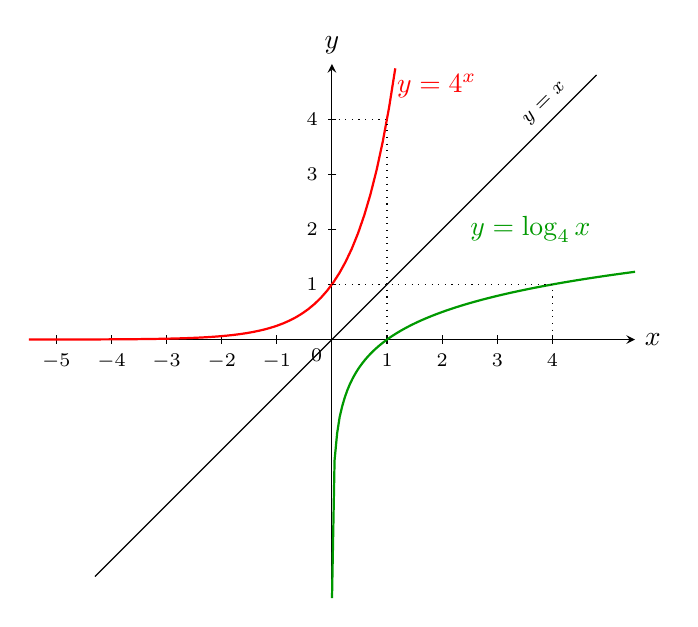
\begin{tikzpicture}[scale=0.7,>=stealth]
  \draw[->] (-5.5,0) -- (5.5,0) node[right] {$x$};
  \draw[->] (0,-4.5) -- (0,5) node[above] {$y$};
  \foreach \x in {-5,-4,-3,-2,-1,1,2,3,4} \draw (\x,0.08) -- (\x,-0.08) node[below] {\scriptsize $\x$};
  \foreach \y in {1,2,3,4} \draw (0.08,\y) -- (-0.08,\y) node[left] {\scriptsize $\y$};
  \node[below left] at (0,0) {\scriptsize $0$};
  \draw (-4.3,-4.3) -- (4.8,4.8) node[pos=0.92,above,sloped] {\scriptsize $y = x$};
  \draw[thick,red,domain=-5.5:1.15,samples=60] plot (\x,{4^\x});
  \draw[thick,green!60!black,domain=0.0015:5.5,samples=120] plot (\x,{ln(\x)/ln(4)});
  \draw[dotted] (0,4) -- (1,4) -- (1,0);
  \draw[dotted] (0,1) -- (4,1) -- (4,0);
  \node[red] at (1.9,4.6) {$y = 4^x$};
  \node[green!60!black] at (3.6,2) {$y = \log_4 x$};
\end{tikzpicture}
\end{center}
តាមក្រាប យើងសង្កេតឃើញថា
\begin{itemize}
  \item តម្លៃ $x$ កើន គេបានតម្លៃត្រូវគ្នានៃ $y = \log_4 x$ កើន
  \item ក្រាបនៃអនុគមន៍ $y = \log_4 x$ កាត់អ័ក្ស $(ox)$ ត្រង់ចំណុច $(1, 0)$ ជានិច្ច
  \item ក្រាបនៃអនុគមន៍ $y = \log_4 x$ និង $y = 4^x$ ឆ្លុះគ្នាធៀបនឹងបន្ទាត់ $y = x$ ។
\end{itemize}
\end{example}

\begin{example}[ឧទាហរណ៍ ខ]
សង់ក្រាបនៃអនុគមន៍ $y = \left(\dfrac{1}{4}\right)^x$, $y = \log_{\frac{1}{4}} x$ និងបន្ទាត់ $y = x$ ។

តារាងតម្លៃត្រូវគ្នានៃ $x$ និង $y$
\[
\begin{array}{|c|c|c|c|c|c|}\hline
x & -2 & -1 & 0 & 1 & 2\\ \hline
y = \left(\frac{1}{4}\right)^x & 16 & 4 & 1 & 0.25 & 0.06\\ \hline
\end{array}
\]
\[
\begin{array}{|c|c|c|c|c|c|}\hline
x & 0.25 & 0.50 & 1 & 2 & 4\\ \hline
y = \log_{\frac{1}{4}} x & 1 & 0.50 & 0 & -0.50 & -1\\ \hline
\end{array}
\]
\begin{center}
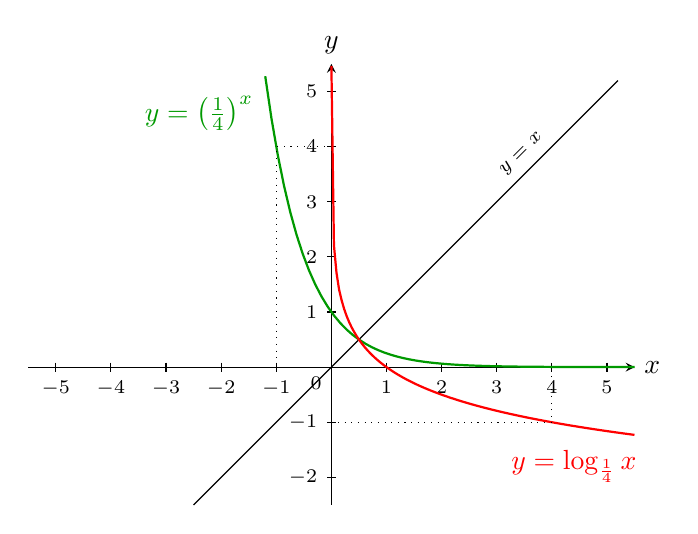
\begin{tikzpicture}[scale=0.7,>=stealth]
  \draw[->] (-5.5,0) -- (5.5,0) node[right] {$x$};
  \draw[->] (0,-2.5) -- (0,5.5) node[above] {$y$};
  \foreach \x in {-5,-4,-3,-2,-1,1,2,3,4,5} \draw (\x,0.08) -- (\x,-0.08) node[below] {\scriptsize $\x$};
  \foreach \y in {-2,-1,1,2,3,4,5} \draw (0.08,\y) -- (-0.08,\y) node[left] {\scriptsize $\y$};
  \node[below left] at (0,0) {\scriptsize $0$};
  \draw (-2.5,-2.5) -- (5.2,5.2) node[pos=0.8,above,sloped] {\scriptsize $y = x$};
  \draw[thick,green!60!black,domain=-1.2:5.5,samples=60] plot (\x,{0.25^\x});
  \draw[thick,red,domain=0.0005:5.5,samples=120] plot (\x,{-ln(\x)/ln(4)});
  \draw[dotted] (0,4) -- (-1,4) -- (-1,0);
  \draw[dotted] (0,-1) -- (4,-1) -- (4,0);
  \node[green!60!black] at (-2.4,4.6) {$y = \left(\frac{1}{4}\right)^x$};
  \node[red] at (4.4,-1.8) {$y = \log_{\frac{1}{4}} x$};
\end{tikzpicture}
\end{center}
តាមក្រាប យើងសង្កេតឃើញថា
\begin{itemize}
  \item តម្លៃ $x$ កើន គេបានតម្លៃត្រូវគ្នានៃ $y = \log_{\frac{1}{4}} x$ ចុះ
  \item ក្រាបនៃអនុគមន៍ $y = \log_{\frac{1}{4}} x$ កាត់អ័ក្ស $(ox)$ ត្រង់ចំណុច $(1, 0)$
  \item ក្រាបនៃអនុគមន៍ $y = \log_{\frac{1}{4}} x$ និង $y = \left(\dfrac{1}{4}\right)^x$ ឆ្លុះគ្នាធៀបនឹងបន្ទាត់ $y = x$ ។
\end{itemize}
\end{example}

\begin{formulaBox}[ជាទូទៅ]
បើ $a > 1$ នោះអនុគមន៍ $y = \log_a x$ ជាអនុគមន៍កើន ។

បើ $0 < a < 1$ នោះអនុគមន៍ $y = \log_a x$ ជាអនុគមន៍ចុះ ។
\end{formulaBox}

ជាសន្និដ្ឋាន អនុគមន៍ $y = \log_a x$ មានក្រាប ៖
\begin{itemize}
  \item បើ $a > 1$ ក្រាបកើនពីឆ្វេងទៅស្តាំ គេថា $y = \log_a x$ ជាអនុគមន៍កើន
  \item បើ $0 < a < 1$ ក្រាបចុះពីឆ្វេងទៅស្តាំ គេថា $y = \log_a x$ ជាអនុគមន៍ចុះ
  \item អនុគមន៍ $y = \log_a x$ មានក្រាបកាត់តាមចំណុចដែលមានកូអរដោនេ $(1, 0)$ ជានិច្ច
  \item អនុគមន៍ $y = \log_a x$ មានដែនកំណត់ $x > 0$ ជានិច្ច
  \item អនុគមន៍ $y = \log_a x$ និង $y = a^x$ ជាអនុគមន៍ច្រាសគ្នា ហើយមានក្រាបឆ្លុះគ្នាធៀបនឹងបន្ទាត់ $y = x$ ។
\end{itemize}

\begin{example}[លំហាត់គំរូ ១]
សង់ក្រាបនៃអនុគមន៍ \quad ក. $y = \log_{10} x$ \qquad ខ. $y = \log_{\frac{1}{10}} x$ ។
\end{example}
\ans
ក. តារាងតម្លៃត្រូវគ្នានៃ $x$ និង $y$
\[
\begin{array}{|c|c|c|c|c|c|}\hline
x & \frac{1}{100} & \frac{1}{10} & 1 & 10 & 100\\ \hline
y = \log_{10} x & -2 & -1 & 0 & 1 & 2\\ \hline
\end{array}
\]
\begin{center}
\begin{tikzpicture}[scale=0.7,>=stealth]
  \draw[->] (-5.5,0) -- (5.6,0) node[right] {$x$};
  \draw[->] (0,-3.3) -- (0,5) node[above] {$y$};
  \foreach \x in {-5,-4,-3,-2,-1,1,2,3,4,5} \draw (\x,0.08) -- (\x,-0.08) node[below] {\scriptsize $\x$};
  \foreach \y in {-3,-2,-1,1,2,3,4} \draw (0.08,\y) -- (-0.08,\y) node[left] {\scriptsize $\y$};
  \node[below left] at (0,0) {\scriptsize $0$};
  \draw[thick,green!60!black,domain=0.001:5.5,samples=150] plot (\x,{ln(\x)/ln(10)});
  \node[green!60!black] at (4.2,1.4) {$y = \log_{10} x$};
\end{tikzpicture}
\end{center}
យើងសង្កេតឃើញថា អនុគមន៍ $y = \log_{10} x$ មានក្រាបកើន ។

ខ. តារាងតម្លៃត្រូវគ្នានៃ $x$ និង $y$
\[
\begin{array}{|c|c|c|c|c|c|}\hline
x & \frac{1}{100} & \frac{1}{10} & 1 & 10 & 100\\ \hline
y = \log_{\frac{1}{10}} x & 2 & 1 & 0 & -1 & -2\\ \hline
\end{array}
\]
\begin{center}
\begin{tikzpicture}[scale=0.7,>=stealth]
  \draw[->] (-5.5,0) -- (5.6,0) node[right] {$x$};
  \draw[->] (0,-3.3) -- (0,5) node[above] {$y$};
  \foreach \x in {-5,-4,-3,-2,-1,1,2,3,4,5} \draw (\x,0.08) -- (\x,-0.08) node[below] {\scriptsize $\x$};
  \foreach \y in {-3,-2,-1,1,2,3,4} \draw (0.08,\y) -- (-0.08,\y) node[left] {\scriptsize $\y$};
  \node[below left] at (0,0) {\scriptsize $0$};
  \draw[thick,green!60!black,domain=0.00002:5.5,samples=200] plot (\x,{-ln(\x)/ln(10)});
  \node[green!60!black] at (4.2,-1.4) {$y = \log_{\frac{1}{10}} x$};
\end{tikzpicture}
\end{center}
យើងសង្កេតឃើញថា អនុគមន៍ $y = \log_{\frac{1}{10}} x$ មានក្រាបចុះ ។

\begin{pro}
សង់ក្រាបនៃអនុគមន៍ \quad ក. $y = \log_7 x$ \qquad ខ. $y = \log_{\frac{1}{7}} x$ ។
\end{pro}

\section{លក្ខណៈក្រាបនៃអនុគមន៍លោការីត}

\begin{example}[ឧទាហរណ៍]
សង់ក្រាបនៃអនុគមន៍ \quad ក. $y = -2 + \log_3 x$ \qquad ខ. $y = \log_3(x - 2)$ \qquad គ. $y = -\log_3 x$ ។
\end{example}

\textbf{ក.} សង់ក្រាបនៃអនុគមន៍ $y = -2 + \log_3 x$ ។ តារាងតម្លៃត្រូវគ្នានៃ $x$ និង $y$
\[
\begin{array}{|c|c|c|c|c|}\hline
x & \frac{1}{3} & 1 & 3 & 9\\ \hline
\log_3 x & -1 & 0 & 1 & 2\\ \hline
y = -2 + \log_3 x & -3 & -2 & -1 & 0\\ \hline
\end{array}
\]
\begin{center}
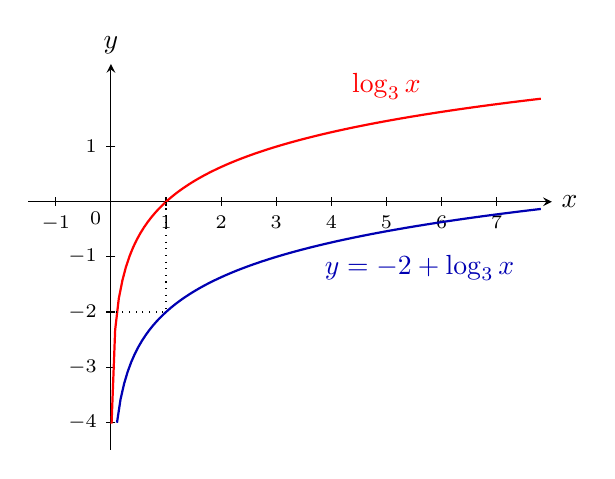
\begin{tikzpicture}[scale=0.7,>=stealth]
  \draw[->] (-1.5,0) -- (8,0) node[right] {$x$};
  \draw[->] (0,-4.5) -- (0,2.5) node[above] {$y$};
  \foreach \x in {-1,1,2,3,4,5,6,7} \draw (\x,0.08) -- (\x,-0.08) node[below] {\scriptsize $\x$};
  \foreach \y in {-4,-3,-2,-1,1} \draw (0.08,\y) -- (-0.08,\y) node[left] {\scriptsize $\y$};
  \node[below left] at (0,0) {\scriptsize $0$};
  \draw[thick,red,domain=0.012:7.8,samples=120] plot (\x,{ln(\x)/ln(3)});
  \draw[thick,blue!70!black,domain=0.11:7.8,samples=120] plot (\x,{-2+ln(\x)/ln(3)});
  \draw[dotted] (1,0) -- (1,-2) -- (0,-2);
  \node[red] at (5,2.1) {$\log_3 x$};
  \node[blue!70!black] at (5.6,-1.2) {$y = -2 + \log_3 x$};
\end{tikzpicture}
\end{center}
ដើម្បីសង់ក្រាបនៃអនុគមន៍ $y = -2 + \log_3 x$ ដំបូងគេសង់ក្រាបនៃអនុគមន៍ $y = \log_3 x$ រួចរំកិលចំនួន $2$ ឯកតាចុះក្រោមស្របអ័ក្ស $(oy)$ គេបានក្រាបនៃអនុគមន៍ $y = -2 + \log_3 x$ ។

\textbf{ខ.} សង់ក្រាបនៃអនុគមន៍ $y = \log_3(x - 2)$ ។ តារាងតម្លៃត្រូវគ្នានៃ $x$ និង $y$
\[
\begin{array}{|c|c|c|c|c|}\hline
x & \frac{7}{3} & 3 & 5 & 11\\ \hline
y = \log_3(x - 2) & -1 & 0 & 1 & 2\\ \hline
\end{array}
\]
\begin{center}
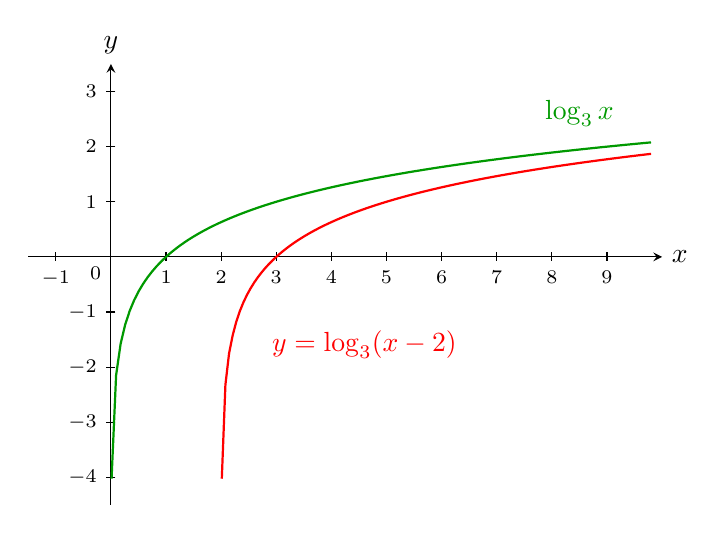
\begin{tikzpicture}[scale=0.7,>=stealth]
  \draw[->] (-1.5,0) -- (10,0) node[right] {$x$};
  \draw[->] (0,-4.5) -- (0,3.5) node[above] {$y$};
  \foreach \x in {-1,1,2,3,4,5,6,7,8,9} \draw (\x,0.08) -- (\x,-0.08) node[below] {\scriptsize $\x$};
  \foreach \y in {-4,-3,-2,-1,1,2,3} \draw (0.08,\y) -- (-0.08,\y) node[left] {\scriptsize $\y$};
  \node[below left] at (0,0) {\scriptsize $0$};
  \draw[thick,green!60!black,domain=0.012:9.8,samples=120] plot (\x,{ln(\x)/ln(3)});
  \draw[thick,red,domain=2.012:9.8,samples=120] plot (\x,{ln(\x-2)/ln(3)});
  \node[green!60!black] at (8.5,2.6) {$\log_3 x$};
  \node[red] at (4.6,-1.6) {$y = \log_3(x - 2)$};
\end{tikzpicture}
\end{center}
ដើម្បីសង់ក្រាបនៃអនុគមន៍ $y = \log_3(x - 2)$ ដំបូងគេសង់ក្រាបនៃអនុគមន៍ $y = \log_3 x$ រួចរំកិលចំនួន $2$ ឯកតា ទៅខាងស្តាំស្របអ័ក្ស $(ox)$ គេបានក្រាបនៃអនុគមន៍ $y = \log_3(x - 2)$ ។

\textbf{គ.} សង់ក្រាបនៃអនុគមន៍ $y = -\log_3 x$ ។ តារាងតម្លៃត្រូវគ្នានៃ $x$ និង $y$
\[
\begin{array}{|c|c|c|c|c|c|}\hline
x & \frac{1}{9} & \frac{1}{3} & 1 & 3 & 9\\ \hline
y = -\log_3 x & 2 & 1 & 0 & -1 & -2\\ \hline
\end{array}
\]
\begin{center}
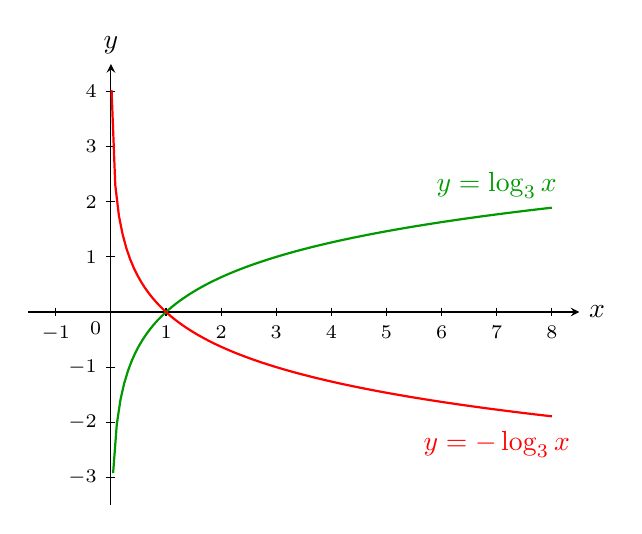
\begin{tikzpicture}[scale=0.7,>=stealth]
  \draw[->] (-1.5,0) -- (8.5,0) node[right] {$x$};
  \draw[->] (0,-3.5) -- (0,4.5) node[above] {$y$};
  \foreach \x in {-1,1,2,3,4,5,6,7,8} \draw (\x,0.08) -- (\x,-0.08) node[below] {\scriptsize $\x$};
  \foreach \y in {-3,-2,-1,1,2,3,4} \draw (0.08,\y) -- (-0.08,\y) node[left] {\scriptsize $\y$};
  \node[below left] at (0,0) {\scriptsize $0$};
  \draw[thick,green!60!black,domain=0.04:8,samples=120] plot (\x,{ln(\x)/ln(3)});
  \draw[thick,red,domain=0.012:8,samples=120] plot (\x,{-ln(\x)/ln(3)});
  \node[green!60!black] at (7,2.3) {$y = \log_3 x$};
  \node[red] at (7,-2.4) {$y = -\log_3 x$};
\end{tikzpicture}
\end{center}
ដើម្បីសង់ក្រាបនៃអនុគមន៍ $y = -\log_3 x$ ដំបូងគេសង់ក្រាបនៃអនុគមន៍ $y = \log_3 x$ រួចគូសក្រាបឆ្លុះរបស់វាធៀបនឹងអ័ក្ស $(ox)$ គេបានក្រាបនៃអនុគមន៍ $y = -\log_3 x$ ។

\begin{formulaBox}[ជាទូទៅ]
\begin{itemize}
  \item ដើម្បីសង់ក្រាបនៃអនុគមន៍ $y = \log_a x + q$ គេត្រូវសង់ក្រាប $y = \log_a x$ រួចធ្វើបម្លែងកិលក្រាបស្របអ័ក្ស $(oy)$ ចំនួន $q$ ឯកតាឡើងលើបើ $q > 0$ ហើយចំនួន $q$ ឯកតា ចុះក្រោមបើ $q < 0$ ។
  \item ដើម្បីសង់ក្រាបនៃអនុគមន៍ $y = \log_a(x - p)$ គេត្រូវសង់ក្រាប $y = \log_a x$ រួចធ្វើបម្លែងកិលក្រាបស្របអ័ក្ស $(ox)$ ចំនួន $p$ ឯកតាទៅខាងស្តាំបើ $p > 0$ ហើយ $p$ ឯកតាទៅខាងឆ្វេងបើ $p < 0$ ។
  \item ដើម្បីសង់ក្រាបនៃអនុគមន៍ $y = -\log_a x$ គេត្រូវសង់ក្រាប $y = \log_a x$ រួចគូសក្រាបឆ្លុះធៀបនឹងអ័ក្ស $(ox)$ គេបានក្រាប $y = -\log_a x$ ។
\end{itemize}
\end{formulaBox}

\begin{pro}
សង់ក្រាបនៃអនុគមន៍
\begin{tasks}(2)
  \task $y = \log_7(x + 3)$
  \task $y = \log_7 x + 3$
  \task $y = -\log_7 x$
  \task $y = \log_2(x - 1)^2$
  \task $y = 2 - \log_2 x^2$ ។
\end{tasks}
\end{pro}

\section{រូបមន្តប្តូរគោល}

ទ្រឹស្តីបទខាងក្រោម អាចឱ្យអ្នកសិក្សាអនុគមន៍លោការីត ប្រើសម្រាប់ប្តូរគោលនៃលោការីតទៅជាគោលដែលគេអាចគណនាបាន ។

\begin{theorem}[រូបមន្តប្តូរគោល]
បើ $a$, $b$ និង $x$ ជាចំនួនពិតវិជ្ជមាន ហើយ $a \ne 1$, $b \ne 1$ គេបាន $\log_a x = \dfrac{\log_b x}{\log_b a}$ ។
\end{theorem}

\textbf{សម្រាយបញ្ជាក់} \ $\log_a x = \dfrac{\log_b x}{\log_b a}$

តាង $M = \log_a x$ គេបាន $a^M = x$ ។ នោះ
\[
\begin{aligned}
\log_b a^M &= \log_b x\\
M\log_b a &= \log_b x
\end{aligned}
\]
នាំឱ្យ $M = \dfrac{\log_b x}{\log_b a}$ ។ យើងទាញបាន $\log_a x = \dfrac{\log_b x}{\log_b a}$ ។

\begin{example}[លំហាត់គំរូ ២]
គណនា
\begin{tasks}(4)
  \task $\log_9 27$
  \task $\log_{27} \dfrac{1}{3}$
  \task $\log_7 27$
  \task $\log_5 125$ ។
\end{tasks}
\end{example}
\ans
\begin{tasks}(2)
  \task $\log_9 27 = \dfrac{\log_3 27}{\log_3 9} = \dfrac{\log_3 3^3}{\log_3 3^2} = \dfrac{3}{2}$
  \task $\log_{27} \dfrac{1}{3} = \log_{3^3} 3^{-1} = -\dfrac{1}{3}$
  \task $\log_7 27 = \dfrac{\log_{10} 27}{\log_{10} 7} \approx 1.6937$
  \task $\log_5 125 = \log_5 5^3 = 3$ ។
\end{tasks}

\begin{pro}
គណនា
\begin{tasks}(3)
  \task $\log_5 625$
  \task $\log_5 346$
  \task $\log_6 4870$ ។
\end{tasks}
\ans
\begin{tasks}(3)
  \task $4$
  \task $\approx 3.63$
  \task $\approx 4.73$ ។
\end{tasks}
\end{pro}

\section{សមីការនិងវិសមីការលោការីត}

\subsection{សមីការលោការីត}

\begin{example}[ឧទាហរណ៍ ១]
បើ $\log_4 x = \log_4 7$ លក្ខខណ្ឌ ៖ សមីការមានន័យកាលណា $x > 0$ នោះ $x = 7$ ។
\end{example}

\begin{example}[ឧទាហរណ៍ ២]
ដោះស្រាយសមីការ $\log_4 x = \dfrac{5}{2}$ ។ លក្ខខណ្ឌ ៖ សមីការមានន័យកាលណា $x > 0$ ។

$\log_4 x = \dfrac{5}{2}$, \ $\log_4 x = \log_4 4^{\frac{5}{2}}$ \ ប្រើរូបមន្ត $\log_a a = 1$

$x = 4^{\frac{5}{2}} = (2^2)^{\frac{5}{2}}$ ព្រោះ $4 = 2^2$ នាំឱ្យ $x = 2^5$ ឬ $x = 32$ ។
\end{example}

\begin{example}[ឧទាហរណ៍ ៣]
ដោះស្រាយសមីការ $6(\log_x 8 + \log_8 x) = 13$ ។

លក្ខខណ្ឌ ៖ សមីការមានន័យកាលណា $x > 0$ និង $x \ne 1$ ។
\[
\begin{gathered}
6\left(\frac{1}{\log_8 x} + \log_8 x\right) = 13\\
\text{ប្រើរូបមន្តប្តូរគោល } \log_x 8 = \frac{1}{\log_8 x}
\end{gathered}
\]
\[
\begin{aligned}
&6 + 6(\log_8 x)^2 = 13\log_8 x \quad \text{គេបាន}\\
&6(\log_8 x)^2 - 13\log_8 x + 6 = 0\\
&(3\log_8 x - 2)(2\log_8 x - 3) = 0\\
&\log_8 x = \frac{2}{3}, \quad \log_8 x = \frac{3}{2}\\
&x = 8^{\frac{2}{3}}, \quad x = 8^{\frac{3}{2}} \Rightarrow x = 4, \quad x = 16\sqrt{2} \text{ ។}
\end{aligned}
\]
\end{example}

\begin{example}[ឧទាហរណ៍ ៤]
ដោះស្រាយសមីការ $\log_9 x + \log_x 9 = \dfrac{5}{2}$ ។

លក្ខខណ្ឌ ៖ សមីការមានន័យកាលណា $x > 0$ និង $x \ne 1$ ។
\[
\begin{aligned}
&\log_9 x + \frac{1}{\log_9 x} = \frac{5}{2}\\
&(\log_9 x)^2 + 1 = \frac{5}{2}\log_9 x\\
&2(\log_9 x)^2 - 5\log_9 x + 2 = 0\\
&(2\log_9 x - 1)(\log_9 x - 2) = 0 \quad \text{សមមូល} \quad \log_9 x = \frac{1}{2}, \ \log_9 x = 2
\end{aligned}
\]
បើ $\log_9 x = \dfrac{1}{2}$ ឬ $x = 9^{\frac{1}{2}} \Rightarrow x = 3$ ។

បើ $\log_9 x = 2$ ឬ $x = 9^2 \Rightarrow x = 81$ ។
\end{example}

\begin{pro}
ដោះស្រាយសមីការ
\begin{tasks}(3)
  \task $\log_9 x = \dfrac{3}{2}$
  \task $\log_{\frac{1}{10}} x = -3$
  \task $\log_x 9 = 2$ ។
\end{tasks}
\ans
\begin{tasks}(3)
  \task $x = 27$
  \task $x = 1000$
  \task $x = 3$ ។
\end{tasks}
\end{pro}

\subsection{វិសមីការលោការីត}

\begin{example}[ឧទាហរណ៍]
ដោះស្រាយវិសមីការ
\begin{enumerate}[a]
  \item $\log_3 x > \log_3 7$ នោះ $x > 7$ ព្រោះគោល $3$ ធំជាង $1$ ។
  \item $\log_{\frac{1}{2}} x > \log_{\frac{1}{2}} 7$ នោះ $0 < x < 7$ ព្រោះគោល $\dfrac{1}{2}$ តូចជាង $1$ ។
\end{enumerate}
\end{example}

\begin{formulaBox}[ជាទូទៅ]
\begin{itemize}
  \item បើ $a > 1$ នោះវិសមីការ $\log_a x > \log_a y$ សមមូល $x > y$ និង $y > 0$
  \item បើ $0 < a < 1$ នោះវិសមីការ $\log_a x > \log_a y$ សមមូល $x < y$ និង $x > 0$ ។
\end{itemize}
\end{formulaBox}

\begin{example}[លំហាត់គំរូ ៣]
ដោះស្រាយវិសមីការខាងក្រោម រួចផ្ទៀងផ្ទាត់
\begin{tasks}(2)
  \task $\log_3(3x - 5) > \log_3(x + 7)$
  \task $\log_{\frac{1}{2}}(2x - 1) \le 2$ ។
\end{tasks}
\end{example}
\ans
\begin{enumerate}[a]
  \item $\log_3(3x - 5) > \log_3(x + 7)$
  \[
  \begin{array}{ll}
  3x - 5 > x + 7 & \text{លក្ខណៈនៃវិសមីការរបស់អនុគមន៍លោការីត}\\
  2x > 12 & \text{លក្ខណៈបូកបន្ថែម ឬដកលើអង្គទាំងពីរនៃវិសមីការ}\\
  x > 6 & \text{ចែកអង្គទាំងពីរនឹង } 2
  \end{array}
  \]
  ផ្ទៀងផ្ទាត់ ៖ $\log_3(3x - 5)$ មានន័យបើ $3x - 5 > 0$ ឬ $x > \dfrac{5}{3}$ ។ \ $\log_3(x + 7)$ មានន័យបើ $x + 7 > 0$ ឬ $x > -7$ ។

  ដូច្នេះវិសមីការមានសំណុំចម្លើយ $x > 6$ ឬ $x \in (6, +\infty)$ ។
  \item $\log_{\frac{1}{2}}(2x - 1) \le 2$

  $\log_{\frac{1}{2}}(2x - 1) \le \log_{\frac{1}{2}}\left(\dfrac{1}{2}\right)^2$ ឬ $2 = \log_{\frac{1}{2}}\left(\dfrac{1}{2}\right)^2$ តាមលក្ខណៈលោការីតនៃគោល

  $2x - 1 \ge \dfrac{1}{4}$ ប្តូរទិសដៅព្រោះគោលស្មើនឹង $\dfrac{1}{2} < 1$, \ $x \ge \dfrac{5}{8}$ ។

  ផ្ទៀងផ្ទាត់ ៖ $\log_{\frac{1}{2}}(2x - 1)$ មានន័យបើ $2x - 1 > 0$ ឬ $x > \dfrac{1}{2}$ ។

  ដូច្នេះ វិសមីការមានសំណុំចម្លើយ $x \ge \dfrac{5}{8}$ ឬ $x \in \left[\dfrac{5}{8}, +\infty\right)$ ។
\end{enumerate}

\begin{pro}
ដោះស្រាយវិសមីការ
\begin{tasks}(3)
  \task $\log_5(x^2 - 6) > \log_5 x$
  \task $\log_{\frac{1}{3}} x < 0$
  \task $\log_x 27 \ge 3$ ។
\end{tasks}
\ans
\begin{tasks}(3)
  \task $x \in (3, +\infty)$
  \task $x > 1$
  \task $x \in (1, 3]$ ។
\end{tasks}
\end{pro}

\section{លោការីតគោល 10 និងលោការីតនេពែ}

\subsection{លោការីតគោល 10}

\begin{example}[ឧទាហរណ៍]
គេឱ្យអនុគមន៍ $y = 10^x$ គេបាន $x = \log_{10}(y)$ ។ កន្សោម $\log_{10}(y)$ ហៅថា ``លោការីតគោល $10$'' ។
\[
\begin{array}{c|cccc}
x & 1 & 10 & 100 & 1000\\ \hline
y = \log_{10} x & 0 & 1 & 2 & 3
\end{array}
\]
\begin{center}
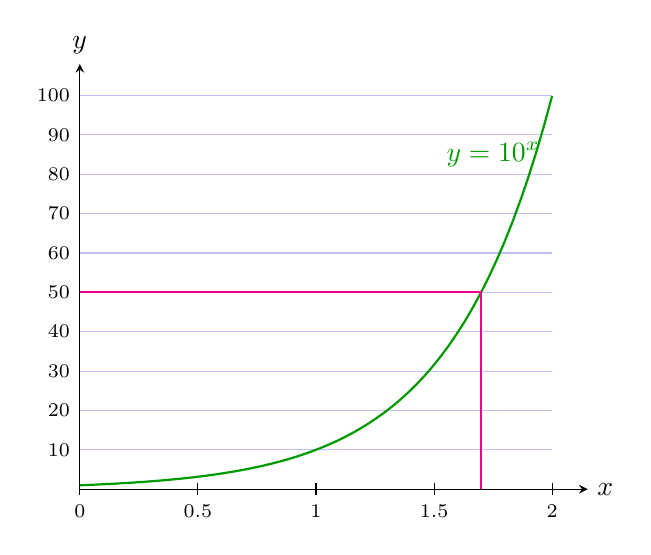
\begin{tikzpicture}[xscale=3,yscale=0.05,>=stealth]
  \foreach \y in {10,20,...,100} \draw[blue!25] (0,\y) -- (2,\y);
  \draw[->] (0,0) -- (2.15,0) node[right] {$x$};
  \draw[->] (0,0) -- (0,108) node[above] {$y$};
  \foreach \x in {0,0.5,1,1.5,2} \draw (\x,1.5) -- (\x,-1.5) node[below] {\scriptsize $\x$};
  \foreach \y in {10,20,...,100} \node[left] at (0,\y) {\scriptsize $\y$};
  \draw[thick,green!60!black,domain=0:2,samples=60] plot (\x,{10^\x});
  \draw[magenta,thick] (0,50) -- ({log10(50)},50) -- ({log10(50)},0);
  \node[green!60!black] at (1.75,85) {$y = 10^x$};
\end{tikzpicture}
\end{center}
\end{example}

\begin{definition}
លោការីតគោល $10$ នៃអថេរមួយ ជាកន្សោមនៃនិទស្សន្តស្វ័យគុណដែលតម្លៃរបស់វាបានមកដោយយក $10$ ជាគោល ហើយត្រូវបានកំណត់សរសេរដោយ $\log_{10} x$ ឬ $\log x$ ។
\end{definition}

\begin{example}[លំហាត់គំរូ ៤]
រកតម្លៃ $x$ ជាអនុគមន៍នៃលោការីតគោល $10$ \quad ក. $10^{2x-3} = 7$ \qquad ខ. $6^{x+2} = 21$ ។
\end{example}
\ans
\begin{enumerate}[a]
  \item $10^{2x-3} = 7$ គេបាន $2x - 3 = \log 7$ នាំឱ្យ $2x = \log 7 + 3$, \ $x = \dfrac{\log 7 + 3}{2}$
  \item $6^{x+2} = 21$ គេបាន $x + 2 = \log_6 21$ នាំឱ្យ $x = \log_6 21 - 2$, \ $x = \dfrac{\log 21}{\log 6} - 2$ ។
\end{enumerate}

\begin{pro}
ដោះស្រាយសមីការ
\begin{tasks}(2)
  \task $\log(40 + y^2) = 2.5$
  \task $\log(y + 18) + \log 5 - \log(2y - 3) = 2$ ។
\end{tasks}
\ans
\begin{tasks}(2)
  \task $y \approx \pm 16.6$
  \task $y = 2$ ។
\end{tasks}
\end{pro}

\subsection{លោការីតនេពែ}

\begin{example}[ឧទាហរណ៍]
គេឱ្យអនុគមន៍ $y = e^x$ ដែល $e$ ជាចំនួនអសនិទាន $e \approx 2.718281828459045\ldots$ នោះគេបាន $x = \log_e(y)$ ។ កន្សោម $\log_e(y)$ ហៅថា ``លោការីតនេពែ'' ។
\end{example}

\begin{definition}
លោការីតនេពែនៃអថេរមួយ ជាកន្សោមនៃនិទស្សន្តស្វ័យគុណដែលតម្លៃរបស់វាបានមកដោយយក $e$ ជាគោល ហើយត្រូវបានកំណត់សរសេរដោយ $\log_e x$ ឬ $\ln x$ ។
\end{definition}

\begin{example}[លំហាត់គំរូ ៥]
រកតម្លៃ $x$ ជាអនុគមន៍នៃលោការីតនេពែ \quad ក. $e^{x-2} = 12$ \qquad ខ. $4e^{2x} + 2 = 18$ ។
\end{example}
\ans
\begin{enumerate}[a]
  \item $e^{x-2} = 12$ គេបាន $x - 2 = \ln 12$ ។ ដូច្នេះ $x = \ln 12 + 2$ ។
  \item $4e^{2x} + 2 = 18$ គេបាន $4e^{2x} = 16$ ឬ $e^{2x} = 4$ ។ ដូច្នេះ $2x = \ln 4$ ឬ $x = \dfrac{\ln 4}{2}$ ។
\end{enumerate}

\begin{pro}
ដោះស្រាយសមីការ \quad ក. $e^{5x+2} = 23$ \qquad ខ. $e^x(2e^x - 1) = 10$ ។
\ans
ក. $x \approx 0.227$ \qquad ខ. $x \approx 0.916$ ។
\end{pro}

\subsection{ក្រាបនៃអនុគមន៍លោការីតគោល 10 និងលោការីតនេពែ}

\[
y = \log_{10} x \Leftrightarrow 10^y = x, \quad \log_{10} x = \log x
\]
\[
y = \log_e x \Leftrightarrow e^y = x, \quad \log_e x = \ln x
\]
\begin{center}
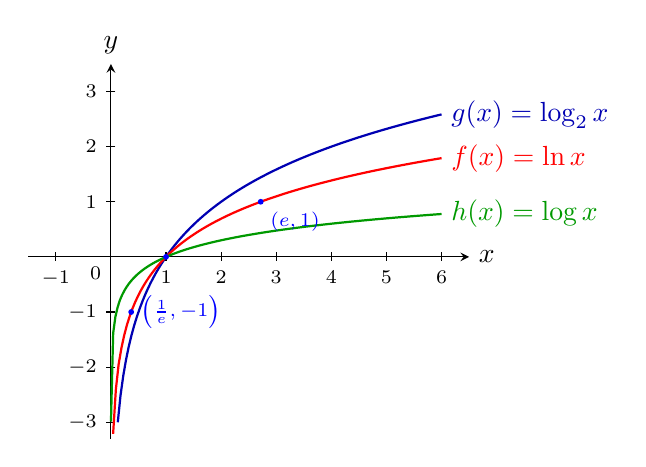
\begin{tikzpicture}[scale=0.7,>=stealth]
  \draw[->] (-1.5,0) -- (6.5,0) node[right] {$x$};
  \draw[->] (0,-3.3) -- (0,3.5) node[above] {$y$};
  \foreach \x in {-1,1,2,3,4,5,6} \draw (\x,0.08) -- (\x,-0.08) node[below] {\scriptsize $\x$};
  \foreach \y in {-3,-2,-1,1,2,3} \draw (0.08,\y) -- (-0.08,\y) node[left] {\scriptsize $\y$};
  \node[below left] at (0,0) {\scriptsize $0$};
  \draw[thick,blue!70!black,domain=0.125:6,samples=120] plot (\x,{ln(\x)/ln(2)});
  \draw[thick,red,domain=0.04:6,samples=120] plot (\x,{ln(\x)});
  \draw[thick,green!60!black,domain=0.001:6,samples=150] plot (\x,{ln(\x)/ln(10)});
  \fill[blue] (1,0) circle (1.5pt);
  \fill[blue] (2.718,1) circle (1.5pt) node[below right] {\scriptsize $(e, 1)$};
  \fill[blue] (0.368,-1) circle (1.5pt) node[right] {\scriptsize $\left(\frac{1}{e}, -1\right)$};
  \node[blue!70!black,right] at (6,2.585) {$g(x) = \log_2 x$};
  \node[red,right] at (6,1.79) {$f(x) = \ln x$};
  \node[green!60!black,right] at (6,0.78) {$h(x) = \log x$};
\end{tikzpicture}
\end{center}

\begin{formulaBox}[ជាទូទៅ]
តាមក្រាប អនុគមន៍លោការីតដែលមានគោលកាន់តែធំ (ចំពោះគោល $a > 1$) នោះអនុគមន៍មានកំណើនកាន់តែយឺត ។
\end{formulaBox}

\section{ការអនុវត្តលើអនុគមន៍លោការីត}

\subsection{តម្លៃកើនតាមឆ្នាំ}

\begin{example}[ឧទាហរណ៍]
មនុស្សម្នាក់បានយកប្រាក់ចំនួន $2\,925\,000$ ៛ ទៅផ្ញើនៅធនាគារដោយទទួលបានអត្រាការប្រាក់ $10\%$ ក្នុងមួយឆ្នាំ ។ ធនាគារទូទាត់ការប្រាក់មួយឆមាសម្តង ។ តើរយៈពេលប៉ុន្មានឆ្នាំ ទើបធ្វើឱ្យប្រាក់របស់គាត់កើនដល់ $3\,705\,000$ ៛?

តាមរូបមន្ត $A = P\left(1 + \dfrac{r}{n}\right)^{nt}$ ដែល $P = 2\,925\,000$ ៛, $r = \dfrac{10}{100} = 0.10$, $A = 3\,705\,000$ ៛, $n = 2$ គេបាន
\[
\begin{aligned}
&3\,705\,000\\
&= 2\,925\,000\left(1 + \frac{0.10}{2}\right)^{2t} \quad \text{ឬ} \quad \frac{3\,705\,000}{2\,925\,000}\\
&= 1.05^{2t}\\
&1.2667 = 1.05^{2t} \quad \text{ឬ} \quad \log 1.2667 = \log 1.05^{2t}\\
&\log 1.2667 = 2t\log 1.05 \quad \text{នាំឱ្យ} \quad t = \frac{\log 1.2667}{2\log 1.05} \approx 2.42
\end{aligned}
\]
ដូច្នេះ ដើម្បីឱ្យប្រាក់របស់គាត់កើនដល់ $3\,705\,000$ ៛ គាត់ត្រូវប្រើពេលអស់ប្រហែល $2.42$ ឆ្នាំ ។
\end{example}

\subsection{តម្លៃថយតាមឆ្នាំ}

\begin{example}[ឧទាហរណ៍]
បើយើងសង្កេតលើរបស់មួយចំនួនដែលយើងជួបប្រទះរាល់ថ្ងៃ យើងឃើញថាមានរបស់ខ្លះឡើងថ្លៃជារៀងរាល់ថ្ងៃ ដូចជា ដី ផ្ទះ ជាដើម ។ល។ ទន្ទឹមនឹងរបស់ដែលកើនតម្លៃរហូត ដូច្នេះ ក៏មានរបស់ខ្លះចុះថ្លៃរហូតដែរ ដូចជារថយន្ត ម៉ូតូ ។ល។ ឧទាហរណ៍ បើយើងទិញរថយន្តថ្មីមួយគ្រឿងតម្លៃ $20\,000$ ដុល្លារ ហើយតម្លៃរថយន្តនេះនឹងចុះថ្លៃ $15\%$ ជារៀងរាល់ឆ្នាំ នោះតារាងតម្លៃរថយន្តចំនួន $4$ ឆ្នាំក្រោយ បង្ហាញដូចតារាងខាងក្រោម ៖
\[
\begin{array}{|c|l|}\hline
\text{ចំនួនឆ្នាំទិញរថយន្ត} & \text{តម្លៃរថយន្តជាដុល្លារ}\\ \hline
0 & 20\,000\\ \hline
1 & 20\,000 - 20\,000 \times 15\% = 17\,000\\ \hline
2 & 17\,000 - 17\,000 \times 15\% = 14\,450\\ \hline
3 & 14\,450 - 14\,450 \times 15\% = 12\,282.5\\ \hline
4 & 12\,282.5 - 12\,282.5 \times 15\% = 10\,440.13\\ \hline
\end{array}
\]
យើងសង្កេតឃើញថា តម្លៃរថយន្តមានការថយចុះជារៀងរាល់ឆ្នាំ ទៅតាមអត្រាភាគរយកំណត់របស់វា ។
\end{example}

\begin{example}[លំហាត់គំរូ ៦]
មនុស្សម្នាក់បានផឹកតែទឹកកកក្រូចឆ្មារមួយកែវ ដែលមានសារជាតិស្ករចំណុះ $130$ មីលីក្រាម ។ បើស្កររលាយចូលក្នុងសារពាង្គកាយក្នុងអត្រា $11\%$ ក្នុងមួយម៉ោង ។ តើរយៈពេលប៉ុន្មានម៉ោង ទើបសារជាតិស្កររលាយចូលក្នុងរាងកាយអស់ពាក់កណ្តាលនៃបរិមាណស្ករដែលមាន?
\end{example}
\ans
ប្រើរូបមន្ត $y = a(1 - r)^t$ ។ ដោយ $y = \dfrac{130}{2} = 65$, $r = \dfrac{11}{100} = 0.11$, $a = 130$ គេបាន
\[
\begin{aligned}
&65 = 130(1 - 0.11)^t\\
&0.89^t = 0.5 \quad \text{ឬ} \quad \log 0.89^t = \log 0.5 \Leftrightarrow t\log 0.89 = \log 0.5\\
&t = \frac{\log 0.5}{\log 0.89} \quad \text{ឬ} \quad t \approx 5.9480 \text{ ។}
\end{aligned}
\]
ដូច្នេះ ដើម្បីឱ្យស្ករជ្រាបចូលក្នុងរាងកាយអស់ពាក់កណ្តាល គេត្រូវប្រើពេលប្រហែល $6$ ម៉ោង ។

\begin{pro}
\begin{enumerate}[a]
  \item ពូសៅបានយកប្រាក់ចំនួន $2\,000\,000$ ៛ ទៅផ្ញើនៅធនាគារដោយទទួលបានអត្រាការប្រាក់ $6\%$ ក្នុងមួយឆ្នាំ ។ តើរយៈពេលប៉ុន្មានឆ្នាំ ទើបប្រាក់របស់គាត់កើនឡើងពីរដង?
  \item គ្រឹះស្ថានបោះពុម្ពនិងចែកផ្សាយបានទិញកុំព្យូទ័រមួយគ្រឿងថ្លៃ $3\,000$ ដុល្លារ ។ បើគេគិតប្រាក់រំលស់ $20\%$ ជារៀងរាល់ឆ្នាំ ចូររកតម្លៃកុំព្យូទ័រក្នុងរយៈពេល $3$ ឆ្នាំក្រោយ ។
  \item តាមការស្រង់ស្ថិតិនាឆ្នាំ $2000$ ប្រទេសចិនមានប្រជាជន $1.26$ ពាន់លាននាក់ ដែលជាចំនួនច្រើនជាងគេបំផុតនៅលើពិភពលោក ។ ប្រទេសដែលមានចំនួនប្រជាជនច្រើនបន្ទាប់ពីប្រទេសចិន គឺប្រទេសឥណ្ឌា ដែលមានចំនួន $1.01$ ពាន់លាននាក់ ។ ចំនួនប្រជាជននៃប្រទេសឥណ្ឌានិងប្រទេសចិន អាចគណនាតាមសមីការ $I(t) = 1.01e^{0.015t}$ និង $C(t) = 1.26e^{0.009t}$ (គេកំណត់ $e = 2.7183$) តាមសមីការគំរូទាំងពីរ តើនៅឆ្នាំណាដែលប្រទេសឥណ្ឌាកើនចំនួនប្រជាជនច្រើនជាងប្រទេសចិន?
\end{enumerate}
\end{pro}

\section*{មេរៀនសង្ខេប ជំពូកទី ២}
\begin{note}[មេរៀនសង្ខេប]
\begin{enumerate}[1]
  \item \textbf{អនុគមន៍អិចស្ប៉ូណង់ស្យែល}
  \begin{itemize}
    \item ស្វ័យគុណ បើ $\underbrace{a \cdot a \cdot a \cdot \ldots \cdot a}_{n \text{ កត្តា}} = a^n$ ដែល $n \in \mathbb{N}$ ។ បើ $a$ និង $b$ ជាចំនួនពិត ហើយ $m$ និង $n$ ជាចំនួនគត់រ៉ឺឡាទីប គេបាន
    \[
\begin{gathered}
a^m \times a^n = a^{m+n}, \quad (a^m)^n = a^{mn},\\
(ab)^n = a^nb^n,\\
\left(\frac{a}{b}\right)^n = \frac{a^n}{b^n} \ (b \ne 0)
\end{gathered}
\]
    \[
\begin{gathered}
\frac{a^m}{a^n} = a^{m-n} \ (a \ne 0),\\
a^0 = 1 \ (a \ne 0),\\
\frac{1}{a^n} = a^{-n} \ (a \ne 0), \ n \in \mathbb{N} \text{ ។}
\end{gathered}
\]
    \item ឫសទី $n$ ៖ បើ $a$ ជាចំនួនពិត $\sqrt[n]{a^n} = |a|$ បើ $n$ ជាចំនួនគត់គូ, $\sqrt[n]{a^n} = a$ បើ $n$ ជាចំនួនគត់សេស ។
    \[
\begin{gathered}
\sqrt[n]{a} \cdot \sqrt[n]{b} = \sqrt[n]{ab},\\
\sqrt[n]{\frac{a}{b}} = \frac{\sqrt[n]{a}}{\sqrt[n]{b}} \ (b \ne 0),\\
\sqrt[n]{a^m} = a^{\frac{m}{n}},\\
\sqrt[n]{\sqrt[k]{a}} = \sqrt[nk]{a},\\
\sqrt[nk]{a^{mk}} = \sqrt[n]{a^m} \text{ ។}
\end{gathered}
\]
    បើ $a > 0$, $a \ne 1$ \ $a^x = a^y$ សមមូល $x = y$ ។
    \item អនុគមន៍អិចស្ប៉ូណង់ស្យែល កំណត់ដោយ $f(x) = a^x$, $x \in \mathbb{R}$, $a > 0$ និង $a \ne 1$ ។
    \item បើ $P$ ប្រាក់ដើម $i$ អត្រាការប្រាក់ប្រចាំឆ្នាំ $n$ ជាចំនួនឆ្នាំ ចំនួនប្រាក់សរុបគឺ $A = P(1 + i)^n$ ។
  \end{itemize}
  \item \textbf{អនុគមន៍លោការីត}
  \begin{itemize}
    \item បើ $(a, b)$ ផ្ទៀងផ្ទាត់ $f(x)$ ហើយ $(b, a)$ ផ្ទៀងផ្ទាត់ $f^{-1}(x)$ នោះ $f^{-1}(x)$ ជាអនុគមន៍ច្រាសនៃអនុគមន៍ $f(x)$ ។
    \item បើអនុគមន៍ពីរច្រាសគ្នា នោះក្រាបនៃអនុគមន៍ទាំងពីរឆ្លុះគ្នាធៀបនឹងបន្ទាត់ $y = x$ ។
    \item បើ $a^x = y$ នោះ $x = \log_a y$, $y > 0$, $a > 0$, $a \ne 1$ ហើយ $f(x) = a^x$ មានអនុគមន៍ច្រាស $f^{-1}(x) = \log_a x$ ។
    \item លក្ខណៈលោការីត ៖ ចំពោះគ្រប់ $x > 0$, $y > 0$, $a > 0$, $a \ne 1$ និង $b > 0$, $b \ne 1$
    \[
\begin{gathered}
\log_a(xy) = \log_a x + \log_a y,\\
\log_a\left(\frac{x}{y}\right) = \log_a x - \log_a y,\\
\log_a x^n = n\log_a x
\end{gathered}
\]
    \[
\begin{gathered}
\log_a b = \frac{1}{\log_b a}, \quad \log_a a = 1, \quad \log_a 1 = 0,\\
\log_a x = \frac{\log_b x}{\log_b a},\\
\log_a a^x = x, \quad a^{\log_a x} = x \text{ ។}
\end{gathered}
\]
  \end{itemize}
\end{enumerate}
\end{note}

\section*{លំហាត់ជំពូកទី ២}
\begin{enumerate}[1]
  \item ដោះស្រាយសមីការអិចស្ប៉ូណង់ស្យែល
  \begin{tasks}(2)
    \task $3^{x^2} = 81^{x-1}$
    \task $9^{(2x-1)^2} = 3^{x+3}$
    \task $2(3)^{2x+3} = 3 - 7(3^x)$
    \task $2^{2x+3} - 2^x = 1 - 2^{x+3}$ ។
  \end{tasks}
  \item បើ $a^x = b^y = (ab)^z$ ។ បង្ហាញថា $xy = z(x + y)$ ។
  \item បើ $2^x = 3^y = 12^z$ ។ បង្ហាញថា $xy = z(x + 2y)$ ។
  \item បើ $a = \sqrt{3} + \sqrt{2}$ និង $b = \sqrt{3} - \sqrt{2}$ ។ បង្ហាញថា $\dfrac{1}{1 + a} + \dfrac{1}{1 + b} = 1$ ។
  \item បើ $a^2 + b^2 = 11ab$ ។ បង្ហាញថា $\log a + \log b = 2\log\left(\dfrac{a - b}{3}\right)$ ។
  \item បើ $\log_x M = a$ និង $\log_y M = b$ ។ បង្ហាញថា $\log_{xy} M = \dfrac{ab}{a + b}$ ។
  \item ដោះស្រាយសមីការលោការីត
  \begin{tasks}(2)
    \task $2 + \log_{10}(2x - 3) = \log_{10} x^2 + \log_{10} 25$
    \task $6(\log_x 8 + \log_8 x) = 13$
    \task $\log_x 9 + \log_9 x = \dfrac{5}{2}$
    \task $\log_9 x + \log_{x^2} 9 = 1$ ។
  \end{tasks}
  \item ដោះស្រាយវិសមីការអិចស្ប៉ូណង់ស្យែល
  \begin{tasks}(3)
    \task $25^x \ge 125^{3x-2}$
    \task $3^x > 27$
    \task $4^x - 6(2^x) + 8 > 0$
    \task $15^x \ge \dfrac{1}{\sqrt[4]{15^3}}$
    \task $\left(\dfrac{1}{5}\right)^x < \sqrt[3]{0.04}$
    \task $(0.3)^x \le \dfrac{100}{9}$ ។
  \end{tasks}
  \item ដោះស្រាយវិសមីការលោការីត
  \begin{tasks}(2)
    \task $\log_{3x-2} x \le 1$
    \task $\log_x^2 x - \log_2 x - 15 < 0$
    \task $\log_{\frac{1}{4}}(3^x - 1) \cdot \log_{\frac{1}{4}}\dfrac{3^x - 1}{16} = \dfrac{3}{4}$
    \task $x \cdot \log_{0.1}(x^2 + x + 1) \ge 0$
    \task $\log_{\frac{x}{5}}(x^2 - 8x + 16) \le 0$
    \task $\log_{x - \frac{9}{2}} \dfrac{x + 4}{2x - 6} \le \log_{x - \frac{9}{2}}(x - 5)$ ។
  \end{tasks}
  \item មនុស្សម្នាក់បានយកប្រាក់ទៅផ្ញើនៅធនាគារអេស៊ីលីដាចំនួន $1\,000\$$ ដោយទទួលបានអត្រាការប្រាក់ $4\%$ ក្នុងមួយឆ្នាំ ។ បើគាត់វិនិយោគប្រាក់នេះតាំងពីឆ្នាំ $1996$ មក តើបច្ចុប្បន្ននេះឆ្នាំ $2007$ គាត់មានប្រាក់សរុបទាំងអស់ប៉ុន្មាននៅធនាគារ?
  \item គេឱ្យអនុគមន៍ $f(x) = a^x$ និងអនុគមន៍ច្រាស $f^{-1}(x) = \log_a x$ ដែល $a$ ជាចំនួនពិតវិជ្ជមាននិង $a \ne 1$ ។
  \begin{enumerate}[a]
    \item រកតម្លៃ $a$ ដើម្បីឱ្យក្រាបនៃអនុគមន៍ $f(x)$ និង $f^{-1}(x)$ កាត់គ្នា ។
    \item រកគ្រប់ចំណុចដែលក្រាបនៃអនុគមន៍ទាំងពីរកាត់គ្នា (ក្នុងសំណួរ ក) ។
  \end{enumerate}
\end{enumerate}

\section*{លំហាត់អនុវត្តន៍}
\begin{enumerate}[1]
  \item រកសមីការនៃអនុគមន៍ច្រាសរបស់អនុគមន៍ខាងក្រោម ៖
  \begin{tasks}(4)
    \task $y = 4x - 3$
    \task $y = 3x^2 + 1$
    \task $x^2 - 3y^2 = 3$
    \task $xy = -6$
    \task $xy^2 = 1$
    \task $\dfrac{x^2}{9} + \dfrac{y^2}{4} = 1$
    \task $y = \dfrac{5}{x}$
    \task $y = \sqrt{x - 2}$ ។
  \end{tasks}
  \item គេឱ្យអនុគមន៍ $f(x) = x - 2$ ។ ចូរកំណត់អនុគមន៍ច្រាស $f^{-1}(x)$ រួចសង់ក្រាបរបស់វា ។
  \item សង់ក្រាបនៃអនុគមន៍ខាងក្រោម ៖
  \begin{tasks}(3)
    \task $y = \log_5 x$
    \task $y = \log_7 x$
    \task $y = \log_{10} x$
    \task $y = \log_{1.5} x$
    \task $y = \log_{0.5} x$
    \task $y = \log_{0.3} x$ ។
  \end{tasks}
  \item បំប្លែងជាទម្រង់លោការីត
  \begin{tasks}(4)
    \task $10^4 = 10000$
    \task $8^{\frac{1}{3}} = 2$
    \task $16^{\frac{1}{4}} = 2$
    \task $5^{-2} = \dfrac{1}{25}$
    \task $4^{-3} = \dfrac{1}{64}$
    \task $10^{0.3010} = 2$
    \task $x^{-a} = y$
    \task $A = k^c$ ។
  \end{tasks}
  \item សម្រួល
  \begin{tasks}(4)
    \task $3^{\log_3 2}$
    \task $5^{\log_5 10}$
    \task $\log_a a^{10}$
    \task $\log_q q^a$
    \task $\log_4 64$
    \task $\log_{10} 0.1$
    \task $\log_{\sqrt{2}} 16$
    \task $\log_{10} 1$ ។
  \end{tasks}
  \item ដោះស្រាយសមីការលោការីត
  \begin{tasks}(3)
    \task $\log_3 x = 3$
    \task $\log_x 16 = 2$
    \task $\log x + \log(x + 9) = 1$
    \task $\log_2 x = -1$
    \task $\log_9 x = \dfrac{1}{2}$
    \task $\log_8 x = \dfrac{1}{3}$
    \task $\log\sqrt[3]{x} = \sqrt{\log x}$
    \task $\log_5\sqrt{x^2 + 1} = \sqrt{1}$
    \task $\log_4(x + 3) + \log_4(x - 3) = 2$
    \task $\log\sqrt[3]{x^2} + \log\sqrt[3]{x^4} = \log 2^{-3}$ ។
  \end{tasks}
  \item ដោះស្រាយវិសមីការលោការីត
  \begin{tasks}(3)
    \task $\log_2 2x \le \log_4(x + 3)$
    \task $\log_3(3x - 5) \ge \log_3(x + 7)$
    \task $\log\dfrac{x^2 - x}{x^2 - 1} < 0$
    \task $\log_{0.5} x^2 < \log_{0.5} 3x$
    \task $\log_5 12 < \log_5(5x - 3)$
    \task $\log(x^2 - 2x + 3) \ge 0$
    \task $\log_8(3x - 1) < \log_8(x + 5)$ ។
  \end{tasks}
  \item ពូសេងយកប្រាក់ $4\,000\,000$ ៛ ទៅផ្ញើវិនិយោគទុន ដោយទទួលបានអត្រាការប្រាក់ $6\%$ ក្នុងមួយឆ្នាំ ។ តើប៉ុន្មានឆ្នាំក្រោយ ទើបប្រាក់របស់គាត់កើនឡើងពីរដង?
  \item មីងសុខាបានទិញរថយន្តថ្មីមួយគ្រឿងថ្លៃ $38\,500$ ដុល្លារ ។ បើរថយន្តចុះថ្លៃក្នុងអត្រា $15\%$ ក្នុងមួយឆ្នាំ ។ តើរយៈពេល $7$ ឆ្នាំក្រោយ រថយន្តគាត់នៅសល់ថ្លៃប៉ុន្មាន?
  \item សរសេរអនុគមន៍ច្រាសនៃអនុគមន៍ខាងក្រោម ៖
  \begin{tasks}(3)
    \task $f(x) = 10^x$
    \task $g(x) = 3^x$
    \task $h(x) = 7^x$
    \task $f(x) = \left(\dfrac{1}{2}\right)^x$
    \task $g(x) = \left(\dfrac{1}{5}\right)^x$
    \task $h(x) = \left(\dfrac{1}{10}\right)^x$ ។
  \end{tasks}
  \item សរសេរអនុគមន៍ច្រាសនៃអនុគមន៍ខាងក្រោម ៖
  \begin{tasks}(3)
    \task $f(x) = \log x$
    \task $g(x) = \log_3 x$
    \task $h(x) = \log_5 x$
    \task $f(x) = \log_{\frac{1}{3}} x$
    \task $g(x) = \log_{\frac{5}{4}} x$
    \task $h(x) = \log_{21} x$ ។
  \end{tasks}
  \item
  \begin{enumerate}[a]
    \item សង់ក្រាបនៃអនុគមន៍អិចស្ប៉ូណង់ស្យែល $f(x) = 5^x$
    \item សង់ក្រាបនៃអនុគមន៍ច្រាសរបស់អនុគមន៍ $f(x) = 5^x$ ក្នុងតម្រុយតែមួយ
    \item សរសេរសមីការអនុគមន៍ច្រាសរបស់អនុគមន៍ខាងលើ ។
  \end{enumerate}
  \item សង់ក្រាបនៃអនុគមន៍ខាងក្រោម ៖
  \begin{tasks}(3)
    \task $f(x) = \log_6 x$
    \task $g(x) = \log_{\frac{1}{6}} x$
    \task $h(x) = \log_{0.8} x$ ។
  \end{tasks}
  \item បង្ហាញថា បើ $f(x) = \log_a x$ នោះ $f(xy) = f(x) + f(y)$ ។
  \item
  \begin{enumerate}[a]
    \item បង្ហាញថា បើ $(x_1, y_1)$ និង $(x_2, y_2)$ ជាចំណុចពីរនៅលើខ្សែកោង $y = \log_a x$ នោះចំណុច $\left(\dfrac{x_1}{x_2}, y_1 - y_2\right)$ ក៏ស្ថិតនៅលើខ្សែកោង $y = \log_a x$ ។
    \item បង្ហាញថា បើ $(x_1, y_1)$ ជាចំណុចនៅលើខ្សែកោង $y = \log_a x$ នោះចំណុច $(x_1^2, 2y_1)$ និងចំណុច $\left(\dfrac{1}{x_1}, -y_1\right)$ ក៏ស្ថិតនៅលើខ្សែកោង $y = \log_a x$ ។
  \end{enumerate}
  \item គេឱ្យអនុគមន៍ $f(x) = a^x$ និងអនុគមន៍ $f^{-1}(x) = \log_a x$ ដែល $a > 0$ ។ រកតម្លៃ $a$ ដើម្បីឱ្យខ្សែកោងនៃអនុគមន៍ $f(x)$ និង $f^{-1}(x)$ កាត់គ្នា ។
  \item គេឱ្យ $f(x) = x - \log_2 x$ ហើយ $g(x) = 2^x$ ។ គណនា \quad ក. $f(g(x))$ \qquad ខ. $g(f(x))$ ។
  \item ដោះស្រាយសមីការនិងផ្ទៀងផ្ទាត់
  \begin{tasks}(2)
    \task $\log_2(2x + 4) - \log_2(x - 1) = 3$
    \task $\log_2 x + \log_4 x = 5$
    \task $\log_5 x + \log_{10} x = 5$
    \task $\log(x + 10) + \dfrac{1}{2}\log x^2 = 2 - \log 4$ ។
  \end{tasks}
  \item រកតម្លៃ $m$ ដើម្បីឱ្យវិសមីការ $1 + \log_5(x^2 + 1) \ge \log_5(mx^2 + 4x + m)$ ផ្ទៀងផ្ទាត់ចំពោះ $\forall x$ ។
  \item រកតម្លៃ $a$ ដើម្បីឱ្យវិសមីការ $\log_{\frac{1}{a+1}}(x^2 + 2) \ge 1$ មានសំណុំឫសចំពោះ $\forall x$ ។
  \item
  \begin{enumerate}[a]
    \item ប្រើ $u = 2^x$ បង្ហាញសមីការ $8^x - 2^{x+2} = 15$ ជាសមីការដឺក្រេទី $3$ នៃ $u$ ។
    \item បង្ហាញថា $u = 3$ ជាឫសតែមួយគត់ដែលជាចំនួនពិតនៃសមីការដឺក្រេទី $3$ ខាងលើ ។
    \item ដោះស្រាយសមីការ $8^x - 2^{x+2} = 15$ ។
  \end{enumerate}
  \item បុរសម្នាក់ទិញម៉ូតូថ្មីមួយគ្រឿង ។ បន្ទាប់ពីរយៈពេល $t$ ដែលជាចំនួនខែនិងតម្លៃរបស់វាតាងដោយ $\$V$ កំណត់ដោយ $V = 10\,000\,e^{-pt}$, $p$ ជាចំនួនថេរ ។
  \begin{enumerate}[a]
    \item រកតម្លៃម៉ូតូនៅពេលដែលបុរសនោះទិញ ដោយដឹងថាតម្លៃសង្ឃឹមទុករបស់ម៉ូតូបន្ទាប់ពីរយៈពេល $12$ ខែស្មើនឹង ។
    \item គណនាតម្លៃសង្ឃឹមទុករបស់ម៉ូតូបន្ទាប់ពីរយៈពេល $18$ ខែ ។
  \end{enumerate}
  \item ដោះស្រាយសមីការនិងប្រព័ន្ធសមីការខាងក្រោម ៖
  \begin{tasks}(2)
    \task $3^{2x+1} - 26(3^x) - 9 = 0$
    \task $\begin{cases} \log p + \log_5 q = 3\\ \log_q p = 2 \end{cases}$ ។
  \end{tasks}
  \item គេមាន $V$ តាងតម្លៃគិតជាដុល្លារនៃផ្ទះមួយកំណត់ដោយសមីការ $V = V_0e^{kt}$ ដែល $V_0$ ដុល្លារ ជាតម្លៃដើមនៃផ្ទះទើបសង់រួច ចំណែកឯ $t$ ជារយៈពេលគិតជាឆ្នាំចាប់តាំងពីការសាងសង់រួចមក ហើយ $k$ គឺជាចំនួនថេរ ។ គណនាតម្លៃ $t$ និង $k$ ក្នុងករណីដូចខាងក្រោម ៖
  \begin{enumerate}[a]
    \item តម្លៃ $k$ បើបន្ទាប់ពីរយៈពេល ឆ្នាំកន្លងមក ផ្ទះមានតម្លៃស្មើនឹងពីរដងតម្លៃដើម
    \item តម្លៃ $t$ ពេលដែលផ្ទះមានតម្លៃស្មើដល់ទៅបីដងតម្លៃដើម ។
  \end{enumerate}
  \item រកតម្លៃ $p$ និង $q$ ដែលជាចំនួនគត់រ៉ឺឡាទីប ចំពោះ $\left(\dfrac{25}{16}\right)^{-\frac{3}{2}} = 2^p \times 5^q$ ។
  \item គេឱ្យ $\log_p X = 4.6$ និង $\log_p Y = 2.3$ ។ គណនាតម្លៃនៃកន្សោមដូចខាងក្រោម ៖ \quad ក. $\log_p X^2Y$ \qquad ខ. $\log_Y X$ ។
  \item គេឱ្យ $2^{2x+2} \times 5^{x-1} = 8^x \times 5^{2x}$ ។ គណនាតម្លៃ $10^x$ ។
  \item គេមានអនុគមន៍ $f$ កំណត់ដោយ $f(x) = \ln x$ ។
  \begin{enumerate}[a]
    \item សង់ក្រាបនៃអនុគមន៍ $f(x) = \ln x$
    \item កំណត់សមីការបន្ទាត់កាត់ក្រាបនៃអនុគមន៍ $f(x) = \ln x$ ដែលចម្លើយរបស់សមីការអាប់ស៊ីសរវាងបន្ទាត់និងក្រាបនៃអនុគមន៍ ជាចម្លើយរបស់សមីការ $x^2e^{x-2} = 1$ ។
  \end{enumerate}
\end{enumerate}
